% $Header:
% $Name:  

\section[P coordinate Global Ocean MITgcm Example]{Global Ocean Simulation at $4^\circ$ Resolution in Pressure
  Coordinates}
\label{www:tutorials}
\label{sect:eg-globalpressure}
\begin{rawhtml}
<!-- CMIREDIR:eg-globalpressure: -->
\end{rawhtml}
\begin{center}
(in directory: {\it verification/tutorial\_global\_oce\_in\_p/})
\end{center}

\bodytext{bgcolor="#FFFFFFFF"}

This example experiment demonstrates using the MITgcm to simulate the
planetary ocean circulation in pressure coordinates, that is, without
making the Boussinesq approximations. The files for this experiment
can be found in the verification directory under tutorial\_global\_oce\_in\_p.
The simulation is configured
with realistic geography and bathymetry on a $4^{\circ} \times
4^{\circ}$ spherical polar grid.  Fifteen levels are used in the
vertical, ranging in thickness from
$50.4089\mbox{\,dbar}\approx50\mbox{\,m}$ at the surface to
$710.33\mbox{\,dbar}\approx690\mbox{\,m}$ at depth, giving a maximum
model depth of $5302.3122\mbox{\,dbar}\approx5200\mbox{\,km}$.  At
this resolution, the configuration can be integrated forward for
thousands of years on a single processor desktop computer.


\subsection{Overview}
\label{www:tutorials}

The model is forced with climatological wind stress data from
Trenberth \cite{trenberth90} and surface flux data from Jiang et~al.\ 
\cite{jiang99}. Climatological data from Levitus \cite{Levitus94} is
used to initialize the model hydrography.  Levitus seasonal
climatology data is also used throughout the calculation to provide
additional air-sea fluxes.  These fluxes are combined with the Jiang
climatological estimates of surface heat flux, resulting in a mixed
boundary condition of the style described in Haney \cite{Haney}.
Altogether, this yields the following forcing applied in the model
surface layer.

\begin{eqnarray}
\label{EQ:eg-global_forcing_pcoord}
\label{EQ:eg-global_forcing_fu_pcoord}
{\cal F}_{u} & = & g\frac{\tau_{x}}{\Delta p_{s}}
\\
\label{EQ:eg-global_forcing_fv_pcoord}
{\cal F}_{v} & = & g\frac{\tau_{y}}{\Delta p_{s}}
\\
\label{EQ:eg-global_forcing_ft_pcoord}
{\cal F}_{\theta} & = & - g\lambda_{\theta} ( \theta - \theta^{\ast} ) 
 - \frac{1}{C_{p} \Delta p_{s}}{\cal Q}
\\
\label{EQ:eg-global_forcing_fs_pcoord}
{\cal F}_{s} & = &
 + g\rho_{FW}\frac{S}{\rho\Delta p_{s}}({\cal E} - {\cal P} - {\cal R})
\end{eqnarray}

\noindent where ${\cal F}_{u}$, ${\cal F}_{v}$, ${\cal F}_{\theta}$,
${\cal F}_{s}$ are the forcing terms in the zonal and meridional
momentum and in the potential temperature and salinity equations
respectively.  The term $\Delta p_{s}$ represents the top ocean layer
thickness in Pa.  It is used in conjunction with a reference density,
$\rho_{FW}$ (here set to $999.8\,{\rm kg\,m^{-3}}$), the surface
salinity, $S$, and a specific heat capacity, $C_{p}$ (here set to
$4000~{\rm J}~^{\circ}{\rm C}^{-1}~{\rm kg}^{-1}$), to convert input
dataset values into time tendencies of potential temperature (with
units of $^{\circ}{\rm C}~{\rm s}^{-1}$), salinity (with units ${\rm
  ppt}~s^{-1}$) and velocity (with units ${\rm m}~{\rm s}^{-2}$).  The
externally supplied forcing fields used in this experiment are
$\tau_{x}$, $\tau_{y}$, $\theta^{\ast}$, $\cal{Q}$ and
$\cal{E}-\cal{P}-\cal{R}$. The wind stress fields ($\tau_x$, $\tau_y$)
have units of ${\rm N}~{\rm m}^{-2}$. The temperature forcing fields
($\theta^{\ast}$ and $Q$) have units of $^{\circ}{\rm C}$ and ${\rm
  W}~{\rm m}^{-2}$ respectively. The salinity forcing fields
($\cal{E}-\cal{P}-\cal{R}$) has units of ${\rm m}~{\rm s}^{-1}$
respectively. The source files and procedures for ingesting these data
into the simulation are described in the experiment configuration
discussion in section \ref{SEC:eg-global-clim_ocn_examp_exp_config}.


\subsection{Discrete Numerical Configuration}
\label{www:tutorials}


Due to the pressure coordinate, the model can only be hydrostatic
\cite{szoeke02}. The domain is discretized with a uniform grid
spacing in latitude and longitude on the sphere $\Delta \phi=\Delta
\lambda=4^{\circ}$, so that there are ninety grid cells in the zonal
and forty in the meridional direction.  The internal model coordinate
variables $x$ and $y$ are initialized according to
\begin{eqnarray}
x=r\cos(\phi),~\Delta x & = &r\cos(\Delta \phi) \\
y=r\lambda,~\Delta y &= &r\Delta \lambda 
\end{eqnarray}

Arctic polar regions are not included in this experiment. Meridionally
the model extends from $80^{\circ}{\rm S}$ to $80^{\circ}{\rm N}$.
Vertically the model is configured with fifteen layers with the
following thicknesses %
\begin{eqnarray*}
  \Delta p_{1} &=& 7103300.720021\mbox{\,Pa},\\
  \Delta p_{2} &=& 6570548.440790\mbox{\,Pa},\\
  \Delta p_{3} &=& 6041670.010249\mbox{\,Pa},\\
  \Delta p_{4} &=& 5516436.666057\mbox{\,Pa},\\
  \Delta p_{5} &=& 4994602.034410\mbox{\,Pa},\\
  \Delta p_{6} &=& 4475903.435290\mbox{\,Pa},\\
  \Delta p_{7} &=& 3960063.245801\mbox{\,Pa},\\
  \Delta p_{8} &=& 3446790.312651\mbox{\,Pa},\\
  \Delta p_{9} &=& 2935781.405664\mbox{\,Pa},\\
  \Delta p_{10}&=& 2426722.705046\mbox{\,Pa},\\
  \Delta p_{11}&=& 1919291.315988\mbox{\,Pa},\\
  \Delta p_{12}&=& 1413156.804970\mbox{\,Pa},\\
  \Delta p_{13}&=& 1008846.750166\mbox{\,Pa},\\
  \Delta p_{14}&=&  705919.025481\mbox{\,Pa},\\
  \Delta p_{15}&=&  504089.693499\mbox{\,Pa},
\end{eqnarray*}
(here the numeric subscript indicates the model level index number,
${\tt k}$; note, that the surface layer has the highest index number 15) to
give a total depth, $H$, of $-5200{\rm m}$. In pressure, this is
$p_{b}^{0}=53023122.566084\mbox{\,Pa}$. 
The implicit free surface form of the pressure equation described in
Marshall et al. \cite{marshall:97a} with the nonlinear extension by
Campin et al. \cite{campin:02} is employed. A Laplacian operator, $\nabla^2$, provides viscous
dissipation. Thermal and haline diffusion is also represented by a Laplacian operator.

Wind-stress forcing is added to the momentum equations in (\ref{EQ:eg-global-model_equations_pcoord}) 
for both the zonal flow, $u$ and the meridional flow $v$, according to equations 
(\ref{EQ:eg-global_forcing_fu_pcoord}) and (\ref{EQ:eg-global_forcing_fv_pcoord}).
Thermodynamic forcing inputs are added to the equations 
in (\ref{EQ:eg-global-model_equations_pcoord}) for
potential temperature, $\theta$, and salinity, $S$, according to equations 
(\ref{EQ:eg-global_forcing_ft_pcoord}) and (\ref{EQ:eg-global_forcing_fs_pcoord}).
This produces a set of equations solved in this configuration as follows:

\begin{eqnarray}
\label{EQ:eg-global-model_equations_pcoord}
\frac{Du}{Dt} - fv + 
  \frac{1}{\rho}\frac{\partial \Phi^{'}}{\partial x} - 
  \nabla_{h}\cdot A_{h}\nabla_{h}u - 
  (g\rho_0)^2\frac{\partial}{\partial p}A_{r}\frac{\partial u}{\partial p} 
 & = &
\begin{cases}
{\cal F}_u & \text{(surface)} \\
0 & \text{(interior)}
\end{cases}
\\
\frac{Dv}{Dt} + fu + 
  \frac{1}{\rho}\frac{\partial \Phi^{'}}{\partial y} - 
  \nabla_{h}\cdot A_{h}\nabla_{h}v - 
  (g\rho_0)^2\frac{\partial}{\partial p}A_{r}\frac{\partial v}{\partial p} 
& = &
\begin{cases}
{\cal F}_v & \text{(surface)} \\
0 & \text{(interior)}
\end{cases}
\\
\frac{\partial p_{b}}{\partial t} + \nabla_{h}\cdot \vec{u}
&=&
0
\\
\frac{D\theta}{Dt} -
 \nabla_{h}\cdot K_{h}\nabla_{h}\theta
 - (g\rho_0)^2\frac{\partial}{\partial p}\Gamma(K_{r})\frac{\partial\theta}{\partial p} 
& = &
\begin{cases}
{\cal F}_\theta & \text{(surface)} \\
0 & \text{(interior)}
\end{cases}
\\
\frac{D s}{Dt} -
 \nabla_{h}\cdot K_{h}\nabla_{h}s
 - (g\rho_0)^2\frac{\partial}{\partial p}\Gamma(K_{r})\frac{\partial S}{\partial p} 
& = &
\begin{cases}
{\cal F}_s & \text{(surface)} \\
0 & \text{(interior)}
\end{cases}
\\
\Phi_{-H}'^{(0)} + \alpha_{0}p_{b}+ \int^{p}_{0}\alpha' dp & = & \Phi'
\end{eqnarray}

\noindent where $u=\frac{Dx}{Dt}=r \cos(\phi)\frac{D \lambda}{Dt}$ and 
$v=\frac{Dy}{Dt}=r \frac{D \phi}{Dt}$ are the zonal and meridional
components of the flow vector, $\vec{u}$, on the sphere. As described
in MITgcm Numerical Solution Procedure \ref{chap:discretization}, the
time evolution of potential temperature, $\theta$, equation is solved
prognostically. The full geopotential height, $\Phi$, is diagnosed by
summing the geopotential height anomalies $\Phi'$ due to bottom
pressure $p_{b}$ and density variations. The integration of the
hydrostatic equation is started at the bottom of the domain. The
condition of $p=0$ at the sea surface requires a time-independent
integration constant for the height anomaly due to density variations
$\Phi_{-H}'^{(0)}$, which is provided as an input field.


\subsection{Experiment Configuration}
\label{www:tutorials}
\label{SEC:eg-globalpressure-config}

The model configuration for this experiment resides under the 
directory {\it tutorial\_examples/global\_ocean\_circulation/}.  
The experiment files 

\begin{itemize}
\item {\it input/data}
\item {\it input/data.pkg}
\item {\it input/eedata},
\item {\it input/topog.bin},
\item {\it input/deltageopotjmd95.bin},
\item {\it input/lev\_s.bin},
\item {\it input/lev\_t.bin},
\item {\it input/trenberth\_taux.bin},
\item {\it input/trenberth\_tauy.bin},
\item {\it input/lev\_sst.bin},
\item {\it input/shi\_qnet.bin},
\item {\it input/shi\_empmr.bin},
\item {\it code/CPP\_EEOPTIONS.h}
\item {\it code/CPP\_OPTIONS.h},
\item {\it code/SIZE.h}. 
\end{itemize}
contain the code customizations and parameter settings for these
experiments. Below we describe the customizations
to these files associated with this experiment.

\subsubsection{Driving Datasets}
\label{www:tutorials}

Figures (\ref{FIG:sim_config_tclim_pcoord}-\ref{FIG:sim_config_empmr_pcoord}) show
the relaxation temperature ($\theta^{\ast}$) and salinity ($S^{\ast}$)
fields, the wind stress components ($\tau_x$ and $\tau_y$), the heat
flux ($Q$) and the net fresh water flux (${\cal E} - {\cal P} - {\cal
  R}$) used in equations
\ref{EQ:eg-global_forcing_fu_pcoord}-\ref{EQ:eg-global_forcing_fs_pcoord}.
The figures also indicate the lateral extent and coastline used in the
experiment.  Figure ({\ref{FIG:model_bathymetry_pcoord}) shows the depth
  contours of the model domain.
\begin{figure}[t]
  \begin{center}
    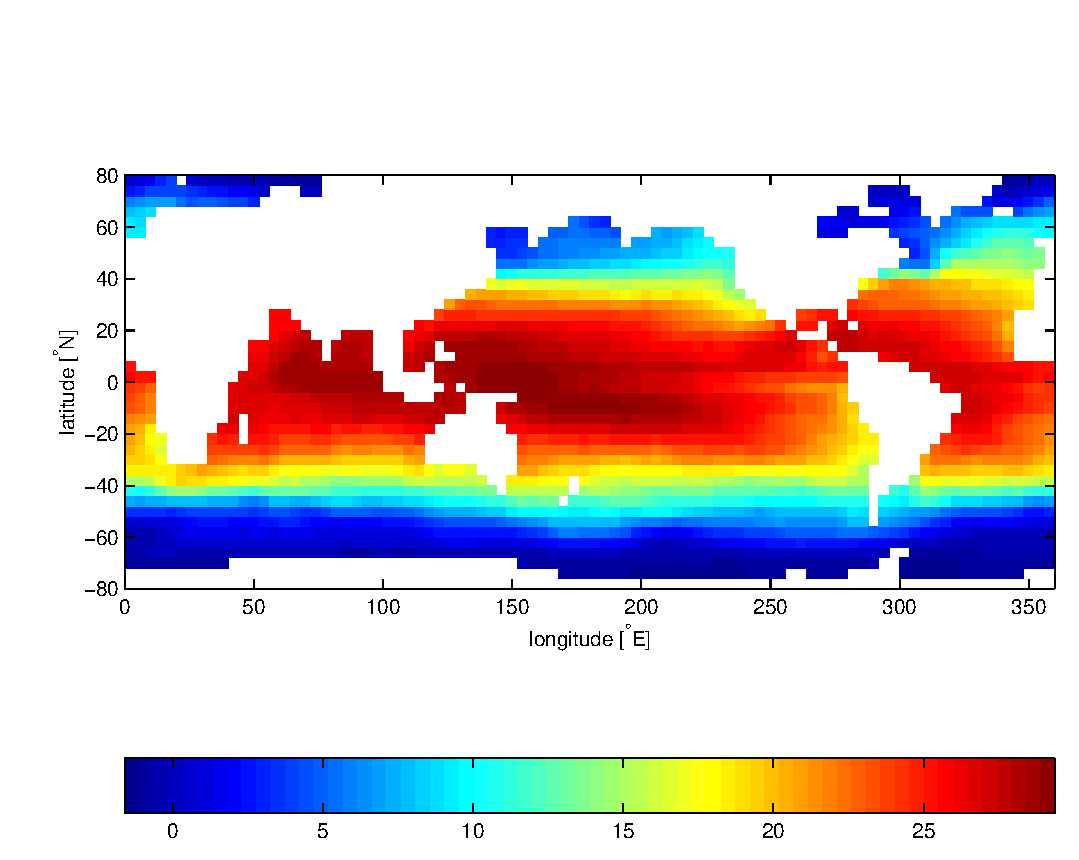
\includegraphics[width=.9\textwidth]{part3/case_studies/ogcm_in_pressure/sst}
    \caption{Annual mean of relaxation temperature [$^{\circ}\mathrm{C}$]}
    \label{FIG:sim_config_tclim_pcoord}
  \end{center}
\end{figure}
\begin{figure}[t]
  \begin{center}
    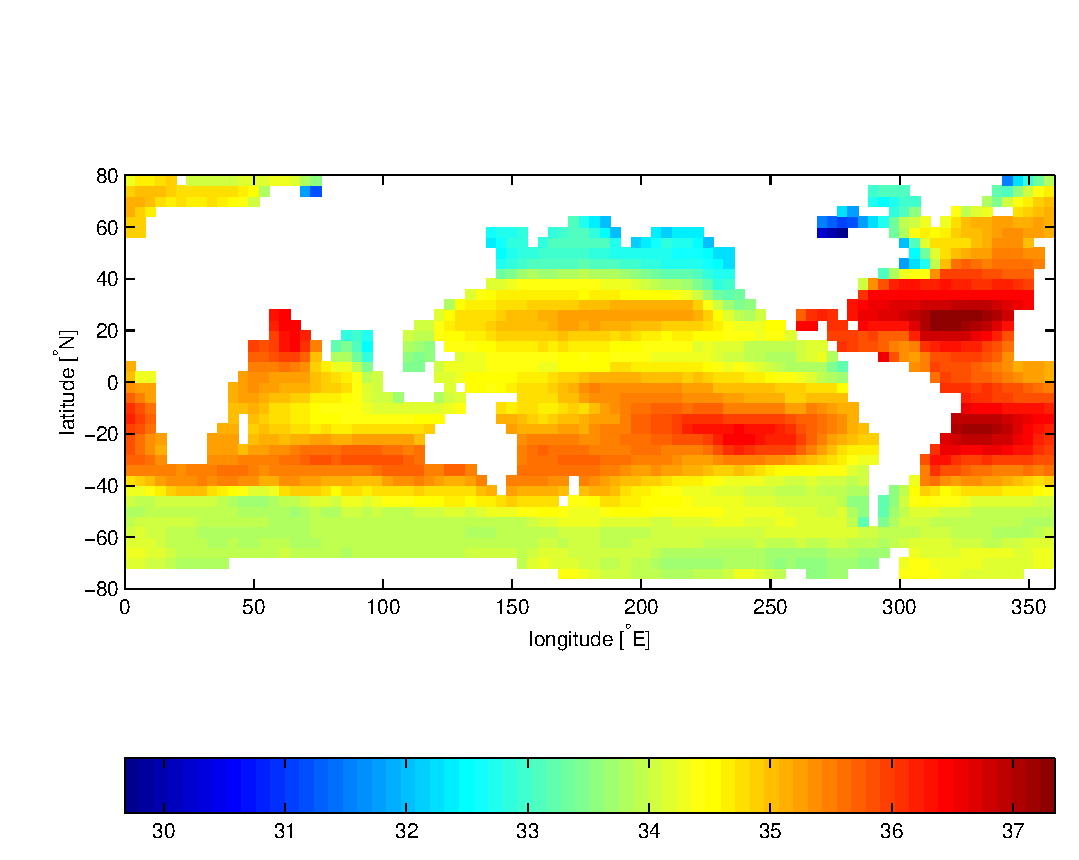
\includegraphics[width=.9\textwidth]{part3/case_studies/ogcm_in_pressure/sss}
    \caption{Annual mean of relaxation salinity [PSU]}
    \label{FIG:sim_config_sclim_pcoord}
  \end{center}
\end{figure}
\begin{figure}[t]
  \begin{center}
    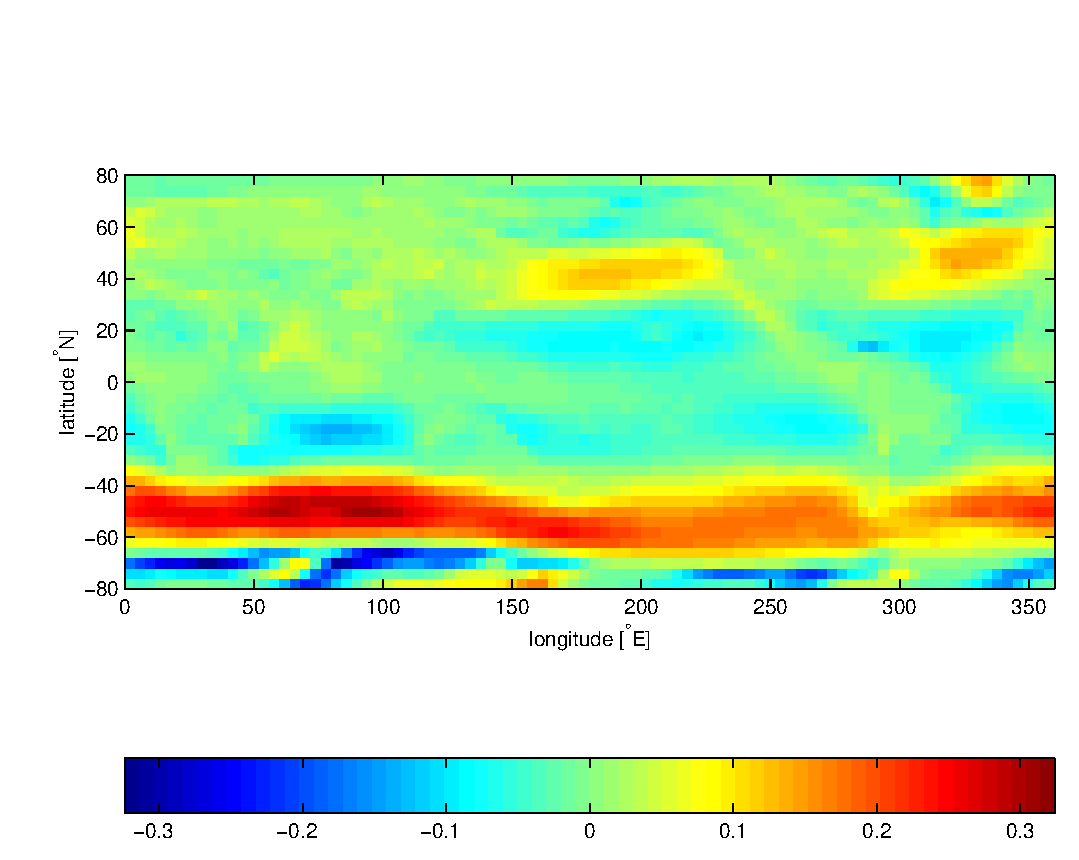
\includegraphics[width=.9\textwidth]{part3/case_studies/ogcm_in_pressure/tx}    
    \caption{Annual mean of zonal wind stress component [Nm\,m$^{-2}$]}
    \label{FIG:sim_config_taux_pcoord}
  \end{center}
\end{figure}
\begin{figure}[t]
  \begin{center}
    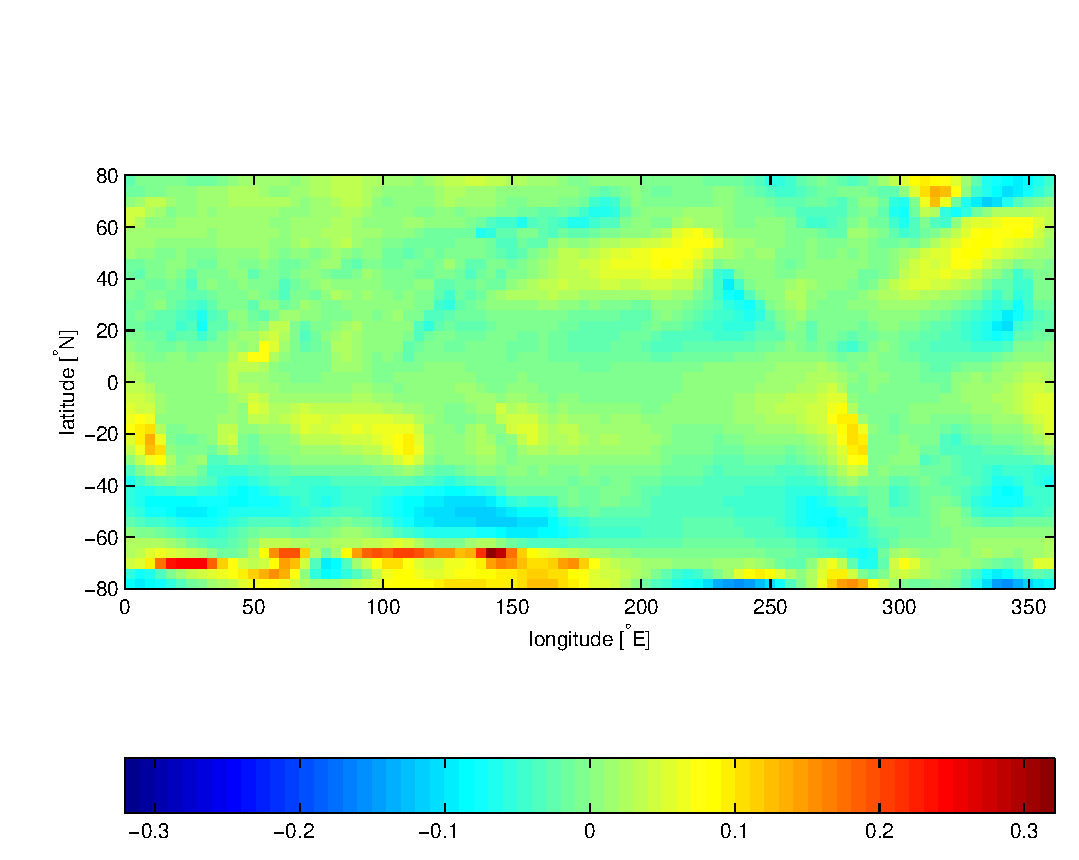
\includegraphics[width=.9\textwidth]{part3/case_studies/ogcm_in_pressure/ty}
    \caption{Annual mean of meridional wind stress component [Nm\,m$^{-2}$]}
    \label{FIG:sim_config_tauy_pcoord}
  \end{center}
\end{figure}
\begin{figure}[t]
  \begin{center}
    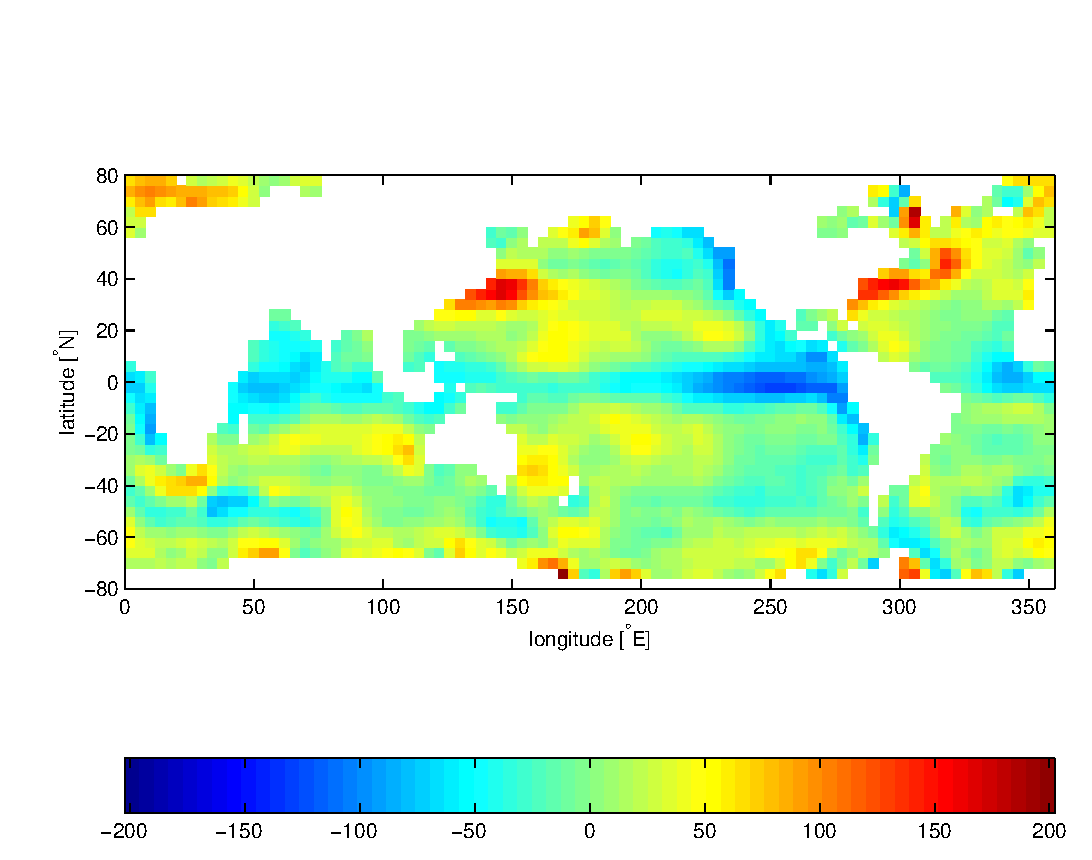
\includegraphics[width=.9\textwidth]{part3/case_studies/ogcm_in_pressure/qnet}
    \caption{Annual mean heat flux [W\,m$^{-2}$]}
    \label{FIG:sim_config_qnet_pcoord}
  \end{center}
\end{figure}
\begin{figure}[t]
  \begin{center}
    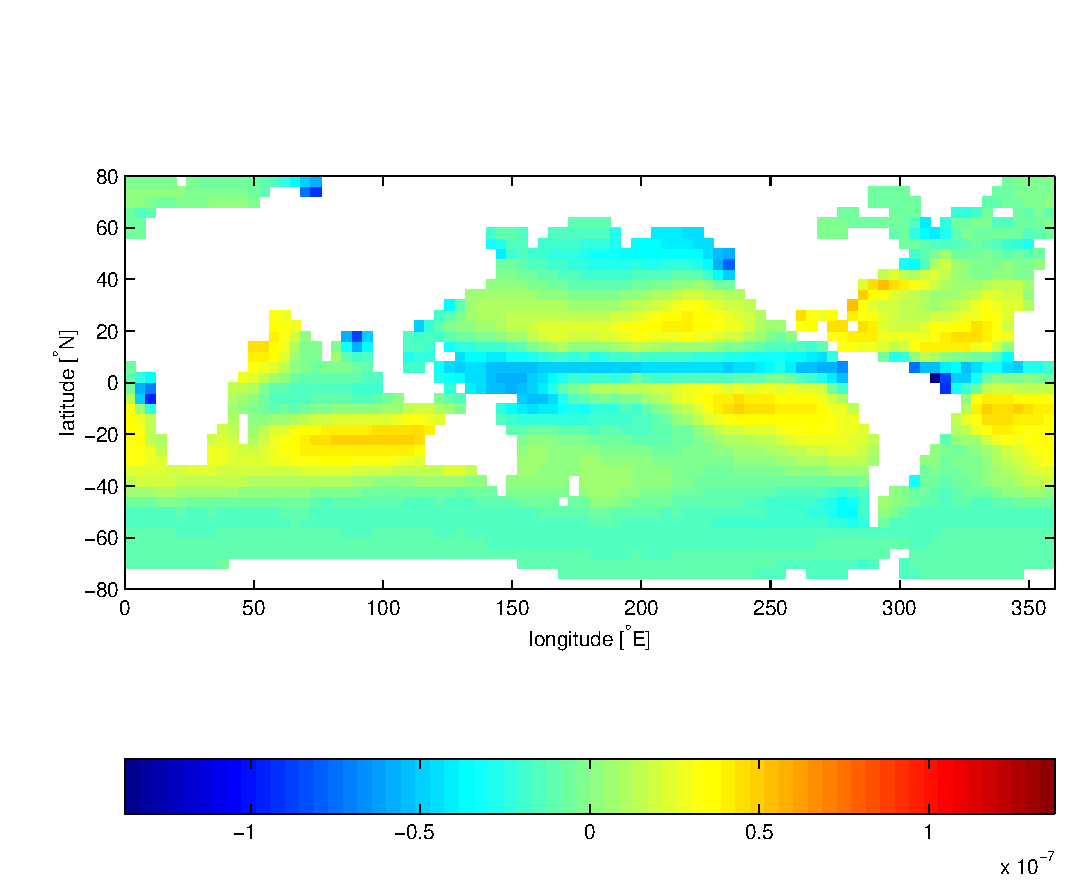
\includegraphics[width=.9\textwidth]{part3/case_studies/ogcm_in_pressure/emp}
    \caption{Annual mean fresh water flux (Evaporation-Precipitation) [m\,s$^{-1}$]}
    \label{FIG:sim_config_empmr_pcoord}
  \end{center}
\end{figure}
\begin{figure}[t]
  \begin{center}
    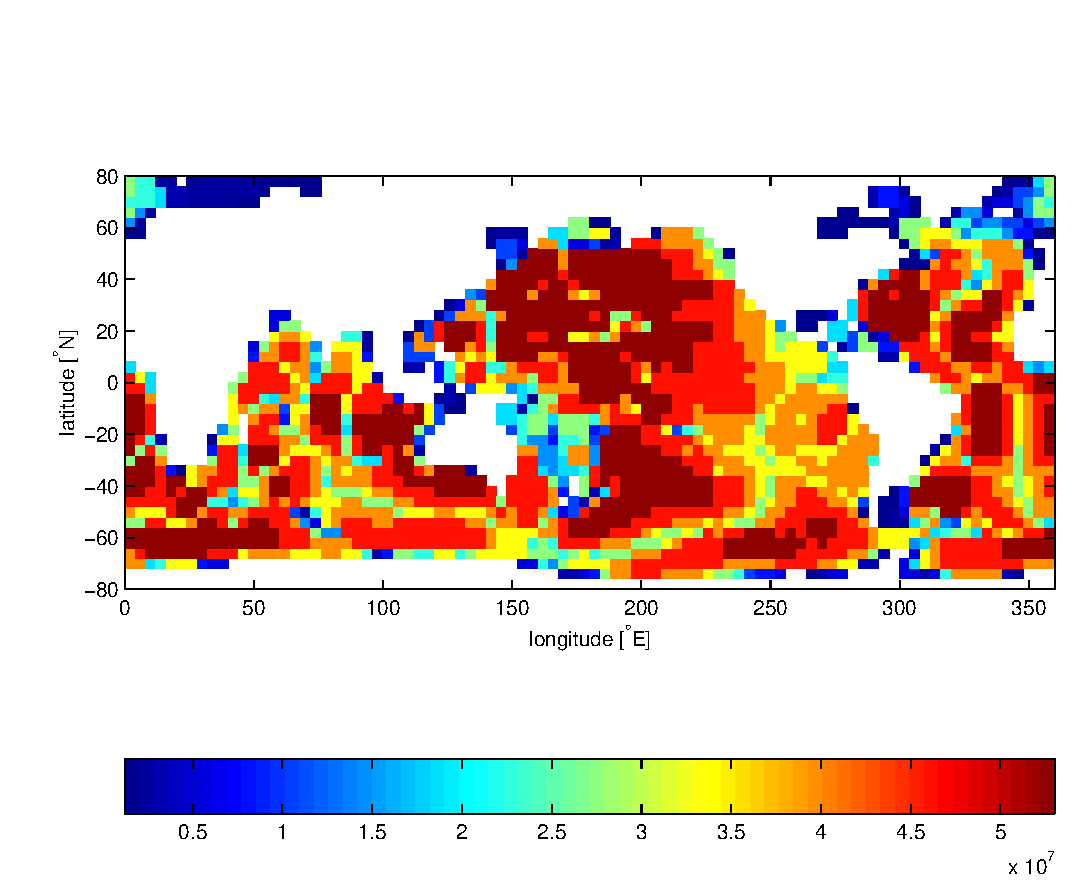
\includegraphics[width=.9\textwidth]{part3/case_studies/ogcm_in_pressure/pb0}
    \caption{Model bathymetry in pressure units [Pa]}
    \label{FIG:model_bathymetry_pcoord}
  \end{center}
\end{figure}

\subsubsection{File {\it input/data}}
\label{www:tutorials}

This file, reproduced completely below, specifies the main parameters 
for the experiment. The parameters that are significant for this configuration
are

\begin{itemize}

\item Line 15, 
\begin{verbatim} viscAr=1.721611620915750E+05, \end{verbatim}
this line sets the vertical Laplacian dissipation coefficient to
$1.72161162091575 \times 10^{5} {\rm Pa^{2}s^{-1}}$. Note that, the factor
$(g\rho)^2$ needs to be included in this line. Boundary conditions
for this operator are specified later. This variable is copied into
model general vertical coordinate variable {\bf viscAr}.

\fbox{
\begin{minipage}{5.0in}
{\it S/R CALC\_DIFFUSIVITY}({\it calc\_diffusivity.F})
\end{minipage}
}

\item Line 9--10, 
\begin{verbatim}
viscAh=3.E5,
no_slip_sides=.TRUE.
\end{verbatim} 
  these lines set the horizontal Laplacian frictional dissipation
  coefficient to $3 \times 10^{5} {\rm m^{2}s^{-1}}$ and specify a
  no-slip boundary condition for this operator, that is, $u=0$ along
  boundaries in $y$ and $v=0$ along boundaries in $x$.

\item Lines 11-13,
\begin{verbatim}
 viscAr =1.721611620915750e5,
#viscAz =1.67E-3,
 no_slip_bottom=.FALSE.,
\end{verbatim}
  These lines set the vertical Laplacian frictional dissipation
  coefficient to $1.721611620915750 \times
  10^{5}\mbox{\,Pa$^{2}$s$^{-1}$}$, which corresponds to
  $1.67\times10^{-3}\mbox{\,m$^{2}$s$^{-1}$}$ in the commented line, and
  specify a free slip boundary condition for this operator, that is,
  $\frac{\partial u}{\partial p}=\frac{\partial v}{\partial p}=0$ at
  $p=p_{b}^{0}$, where $p_{b}^{0}$ is the local bottom pressure of the
  domain at rest. Note that, the factor $(g\rho)^2$ needs to be
  included in this line.

\item Line 14,
\begin{verbatim}
 diffKhT=1.E3,
\end{verbatim}
  this line sets the horizontal diffusion coefficient for temperature
  to $1000\,{\rm m^{2}s^{-1}}$. The boundary condition on this
  operator is $\frac{\partial}{\partial x}=\frac{\partial}{\partial
    y}=0$ on all boundaries.

\item Line 15--16,
\begin{verbatim}
 diffKrT=5.154525811125000e3,
#diffKzT=0.5E-4,
\end{verbatim}
  this line sets the vertical diffusion coefficient for temperature to
  $5.154525811125 \times 10^{3}\,{\rm Pa^{2}s^{-1}}$, which
  corresponds to $5\times10^{-4}\mbox{\,m$^{2}$s$^{-1}$}$ in the commented
  line. Note that, the factor $(g\rho)^2$ needs to be included in this
  line. The boundary condition on this operator is
  $\frac{\partial}{\partial p}=0$ at both the upper and lower
  boundaries.

\item Line 17--19,
\begin{verbatim}
 diffKhS=1.E3,
 diffKrS=5.154525811125000e3,
#diffKzS=0.5E-4,
\end{verbatim}
These lines set the same values for the diffusion coefficients for
salinity as for temperature.

\item Line 20--22,
\begin{verbatim}
 implicitDiffusion=.TRUE.,
 ivdc_kappa=1.030905162225000E9,
#ivdc_kappa=10.0,
\end{verbatim}
Select implicit diffusion as a convection scheme and set coefficient
for implicit vertical diffusion to $1.030905162225\times10^{9}\,{\rm
  Pa^{2}s^{-1}}$, which corresponds to $10\mbox{\,m$^{2}$\,s$^{-1}$}$.

\item Line 23-24,
\begin{verbatim}
 gravity=9.81,
 gravitySign=-1.D0,
\end{verbatim}
  These lines set the gravitational acceleration coefficient to
  $9.81{\rm m}{\rm s}^{-1}$ and define the upward direction relative
  to the direction of increasing vertical coordinate (in pressure
  coordinates, up is in the direction of decreasing pressure)
\item Line 25,
\begin{verbatim}
 rhoNil=1035.,
\end{verbatim}
  sets the reference density of sea water to $1035\mbox{\,kg\,m$^{-3}$}$.\\
\fbox{
\begin{minipage}{5.0in}
{\it S/R CALC\_PHI\_HYD}~({\it calc\_phi\_hyd.F})\\
{\it S/R INI\_CG2D}~({\it ini\_cg2d.F})\\
{\it S/R INI\_CG3D}~({\it ini\_cg3d.F})\\
{\it S/R INI\_PARMS}~({\it ini\_parms.F})\\
{\it S/R SOLVE\_FOR\_PRESSURE}~({\it solve\_for\_pressure.F})
\end{minipage}
}

\item Line 28
\begin{verbatim}
 eosType='JMD95P',
\end{verbatim}
  Selects the full equation of state according to Jackett and McDougall
  \cite{jackett95}. The only other sensible choice is the equation of
  state by McDougall et al. \cite{mcdougall03}, 'MDJFW'. All other
  equations of state do not make sense in this configuration.\\
  \fbox{
    \begin{minipage}{5.0in}
      {\it S/R FIND\_RHO}~({\it find\_rho.F})\\
      {\it S/R FIND\_ALPHA}~({\it find\_alpha.F})
    \end{minipage}
    }

\item Line 28-29,
\begin{verbatim}
 rigidLid=.FALSE., 
 implicitFreeSurface=.TRUE., 
\end{verbatim}
  Selects the barotropic pressure equation to be the implicit free
  surface formulation.
\item Line 30
\begin{verbatim}
 exactConserv=.TRUE.,
\end{verbatim}
  Select a more accurate conservation of properties at the surface
  layer by including the horizontal velocity divergence to update the
  free surface.
\item Line 31--33
\begin{verbatim}
 nonlinFreeSurf=3,
 hFacInf=0.2,
 hFacSup=2.0,
\end{verbatim}
  Select the nonlinear free surface formulation and set lower and
  upper limits for the free surface excursions.
\item Line 34
\begin{verbatim}
 useRealFreshWaterFlux=.FALSE.,
\end{verbatim}
  Select virtual salt flux boundary condition for salinity. The
  freshwater flux at the surface only affect the surface salinity, but 
  has no mass flux associated with it

\item Line 35--36,
\begin{verbatim}
 readBinaryPrec=64,
 writeBinaryPrec=64,
\end{verbatim}
  Sets format for reading binary input datasets and 
  writing binary output datasets holding model fields to
  use 64-bit representation for floating-point numbers.\\
  \fbox{
    \begin{minipage}{5.0in}
      {\it S/R READ\_WRITE\_FLD}~({\it read\_write\_fld.F})\\
      {\it S/R READ\_WRITE\_REC}~({\it read\_write\_rec.F})
    \end{minipage}
    }

\item Line 42,
\begin{verbatim}
 cg2dMaxIters=200,
\end{verbatim}
  Sets maximum number of iterations the two-dimensional, conjugate
  gradient solver will use, {\bf irrespective of convergence 
    criteria being met}.\\
  \fbox{
    \begin{minipage}{5.0in}
      {\it S/R CG2D}~({\it cg2d.F})
    \end{minipage}
    }

\item Line 43,
\begin{verbatim}
cg2dTargetResidual=1.E-13,
\end{verbatim}
  Sets the tolerance which the two-dimensional, conjugate
  gradient solver will use to test for convergence in equation 
  \ref{EQ:congrad_2d_resid} to $1 \times 10^{-9}$.
  Solver will iterate until 
  tolerance falls below this value or until the maximum number of
  solver iterations is reached.\\
  \fbox{
    \begin{minipage}{5.0in}
      {\it S/R CG2D}~({\it cg2d.F})
    \end{minipage}
    }

\item Line 48,
\begin{verbatim}
startTime=0,
\end{verbatim}
Sets the starting time for the model internal time counter.
When set to non-zero this option implicitly requests a 
checkpoint file be read for initial state.
By default the checkpoint file is named according to
the integer number of time steps in the {\bf startTime} value.
The internal time counter works in seconds.

\item Line 49--50,
\begin{verbatim}
 endTime=8640000.,
#endTime=62208000000,
\end{verbatim}
  Sets the time (in seconds) at which this simulation will terminate.
  At the end of a simulation a checkpoint file is automatically
  written so that a numerical experiment can consist of multiple
  stages.  The commented out setting for endTime is for a 2000 year
  simulation.

\item Line 51--53,
\begin{verbatim}
 deltaTmom      =   1200.0,
 deltaTtracer   = 172800.0,
 deltaTfreesurf = 172800.0,
\end{verbatim}
  Sets the timestep $\delta t_{v}$ used in the momentum equations to
  $20~{\rm mins}$ and the timesteps $\delta t_{\theta}$ in the tracer
  equations and $\delta t_{\eta}$ in the implicit free surface
  equation to $48\mbox{\,hours}$.  See section
  \ref{SEC:mom_time_stepping}.\\
\fbox{
\begin{minipage}{5.0in}
{\it S/R TIMESTEP}({\it timestep.F}) \\
{\it S/R INI\_PARMS}({\it ini\_parms.F})\\
{\it S/R MOM\_FLUXFORM}({\it mom\_fluxform.F}) \\
{\it S/R TIMESTEP\_TRACER}({\it timestep\_tracer.F})
\end{minipage}
}

\item Line 55,
\begin{verbatim}
 pChkptFreq  =3110400000.,
\end{verbatim}
write a pick-up file every 100 years of integration.

\item Line 56--58
\begin{verbatim}
 dumpFreq    = 3110400000.,
 taveFreq    = 3110400000.,
 monitorFreq =   31104000.,
\end{verbatim}
  write model output and time-averaged model output every 100 years,
  and monitor statisitics every year.

\item Line 59--61
\begin{verbatim}
 periodicExternalForcing=.TRUE.,
 externForcingPeriod=2592000.,
 externForcingCycle=31104000.,
\end{verbatim}
  Allow periodic external forcing, set forcing period, during which
  one set of data is valid, to 1 month and the repeat cycle to 1 year.\\
\fbox{
\begin{minipage}{5.0in}
{\it S/R EXTERNAL\_FORCING\_SURF}({\it external\_forcing\_surf.F})
\end{minipage}
}
\item Line 62
\begin{verbatim}
 tauThetaClimRelax=5184000.0,
\end{verbatim}
  Set the restoring timescale to 2 months.\\
\fbox{
\begin{minipage}{5.0in}
{\it S/R EXTERNAL\_FORCING\_SURF}({\it external\_forcing\_surf.F})
\end{minipage}
}

\item Line 63
\begin{verbatim}
 abEps=0.1,
\end{verbatim}
  Adams-Bashford factor (see section \ref{sect:adams-bashforth})

\item Line 68--69
\begin{verbatim}
 usingCartesianGrid=.FALSE.,
 usingSphericalPolarGrid=.TRUE.,
\end{verbatim}
  Select spherical grid.
\item Line 70--71
\begin{verbatim}
 dXspacing=4.,
 dYspacing=4.,
\end{verbatim}
Set the horizontal grid spacing in degrees spherical distance.
\item Line 72
\begin{verbatim}
 Ro_SeaLevel=53023122.566084,
\end{verbatim}
specifies the total height (in $r$-units, i.e., pressure units) of the
sea surface at rest. This is a reference value.
\item Line 73
\begin{verbatim}
 groundAtK1=.TRUE.,
\end{verbatim}
specifies the reversal of the vertical indexing. The vertical index is 
1 at the bottom of the doman and maximal (i.e., 15) at the surface.
\item Line 74--78
\begin{verbatim}
 delR=7103300.720021, \ldots 
\end{verbatim}
  set the layer thickness in pressure units, starting with the bottom
  layer.

\item Line 84--93,
\begin{verbatim}
 bathyFile='topog.box'
 ploadFile='deltageopotjmd95.bin'
 hydrogThetaFile='lev_t.bin',
 hydrogSaltFile ='lev_s.bin',
 zonalWindFile  ='trenberth_taux.bin',
 meridWindFile  ='trenberth_tauy.bin',
 thetaClimFile  ='lev_sst.bin',
 surfQFile      ='shi_qnet.bin',
 EmPmRFile      ='shi_empmr.bin',
\end{verbatim}
  This line specifies the names of the files holding the bathymetry
  data set, the
  time-independent geopotential height anomaly at the bottom, initial
  conditions of temperature and salinity, wind stress forcing fields,
  sea surface temperature climatology, heat flux, and fresh water flux
  (evaporation minus precipitation minus run-off) at the surface. 
  See file descriptions in section \ref{SEC:eg-globalpressure-config}.

\end{itemize}

\noindent other lines in the file {\it input/data} are standard values
that are described in the MITgcm Getting Started and MITgcm Parameters
notes.

\begin{small}
% $Header: /u/gcmpack/manual/s_examples/baroclinic_gyre/input/data.tex,v 1.1.1.1 2001/08/08 16:15:46 adcroft Exp $
% $Name:  $

\begin{verbatim}
     1	# Model parameters
     2	# Continuous equation parameters
     3	 &PARM01
     4	 tRef=20.,10.,8.,6.,
     5	 sRef=10.,10.,10.,10.,
     6	 viscAz=1.E-2,
     7	 viscAh=4.E2,
     8	 no_slip_sides=.FALSE.,
     9	 no_slip_bottom=.TRUE.,
    10	 diffKhT=4.E2,
    11	 diffKzT=1.E-2,
    12	 beta=1.E-11,
    13	 tAlpha=2.E-4,
    14	 sBeta =0.,
    15	 gravity=9.81,
    16	 rigidLid=.FALSE.,
    17	 implicitFreeSurface=.TRUE.,
    18	 eosType='LINEAR',
    19	 readBinaryPrec=64,
    20	 &
    21	# Elliptic solver parameters
    22	 &PARM02
    23	 cg2dMaxIters=1000,
    24	 cg2dTargetResidual=1.E-13,
    25	 &
    26	# Time stepping parameters
    27	 &PARM03
    28	 startTime=0.,
    29	 endTime=12000., 
    30	 deltaTmom=1200.0,
    31	 deltaTtracer=1200.0,
    32	 abEps=0.1,
    33	 pChkptFreq=17000.0,
    34	 chkptFreq=0.0,
    35	 dumpFreq=2592000.0,
    36	 &
    37	# Gridding parameters
    38	 &PARM04
    39	 usingCartesianGrid=.FALSE.,
    40	 usingSphericalPolarGrid=.TRUE.,
    41	 phiMin=0.,
    42	 delX=60*1.,
    43	 delY=60*1.,
    44	 delZ=500.,500.,500.,500.,
    45	 &
    46	 &PARM05
    47	 bathyFile='topog.box',
    48	 hydrogThetaFile=,
    49	 hydrogSaltFile=,
    50	 zonalWindFile='windx.sin_y',
    51	 meridWindFile=,
    52	 &
\end{verbatim}

\end{small}

\subsubsection{File {\it input/data.pkg}}
\label{www:tutorials}

This file uses standard default values and does not contain
customisations for this experiment.

\subsubsection{File {\it input/eedata}}
\label{www:tutorials}

This file uses standard default values and does not contain
customisations for this experiment.

\subsubsection{File {\it input/topog.bin}}
\label{www:tutorials}

This file is a two-dimensional ($x,y$) map of
depths. This file is assumed to contain 64-bit binary numbers giving
the depth of the model at each grid cell, ordered with the x
coordinate varying fastest. The points are ordered from low
coordinate to high coordinate for both axes. The units and
orientation of the depths in this file are the same as used in the
MITgcm code (Pa for this experiment). In this experiment, a depth of
$0\mbox{\,Pa}$ indicates a land point wall and a depth of
$>0\mbox{\,Pa}$ indicates open ocean.

\subsubsection{File {\it input/deltageopotjmd95.box}}
\label{www:tutorials}

The file contains 12 identical two dimensional maps ($x,y$) of
geopotential height anomaly at the bottom at rest. The values have
been obtained by vertically integrating the hydrostatic equation with
the initial density field (from {\it input/lev\_t/s.bin}). This file
has to be consitent with the temperature and salinity field at rest
and the choice of equation of state!

\subsubsection{File {\it input/lev\_t/s.bin}}
\label{www:tutorials}

The files {\it input/lev\_t/s.bin} specify the initial conditions for
temperature and salinity for every grid point in a three dimensional
array ($x,y,z$). The data are obtain by interpolating Levitus
\cite{Levitus94} monthly mean values for January onto the model
grid. Keep in mind, that the first index corresponds to the bottom
layer and highest index to the surface layer.

\subsubsection{File {\it input/trenberth\_taux/y.bin}}
\label{www:tutorials}

Each of the {\it input/trenberth\_taux/y.bin} files specifies 12
two-dimensional ($x,y,t$) maps of zonal and meridional wind stress
values, $\tau_{x}$ and $\tau_{y}$, that is monthly mean values from
Trenberth \cite{trenberth90}. The units used are $Nm^{-2}$.

\subsubsection{File {\it input/lev\_sst.bin}}
\label{www:tutorials}

The file {\it input/lev\_sst.bin} contains 12 monthly surface
temperature climatologies from Levitus \cite{Levitus94} in a three
dimensional array ($x,y,t$).

\subsubsection{File {\it input/shi\_qnet/empmr.bin}}
\label{www:tutorials}

The files {\it input/shi\_qnet/empmr.bin} contain 12 monthly surface
fluxes of heat (qnet) and freshwater (empmr) by Jiang et al.
\cite{jiang99} in three dimensional arrays ($x,y,t$). Both fluxes are
normalized so that of one year there is no net flux into the
ocean. The freshwater flux is actually constant in time.

\subsubsection{File {\it code/SIZE.h}}
\label{www:tutorials}

Three lines are customized in this file for the current experiment

\begin{itemize}

\item Line 39, 
\begin{verbatim} sNx=90, \end{verbatim} this line sets
the lateral domain extent in grid points for the
axis aligned with the x-coordinate.

\item Line 40, 
\begin{verbatim} sNy=40, \end{verbatim} this line sets
the lateral domain extent in grid points for the
axis aligned with the y-coordinate.

\item Line 49, 
\begin{verbatim} Nr=15,   \end{verbatim} this line sets
the vertical domain extent in grid points.

\end{itemize}

\begin{small}
\begin{verbatim}
     1	C     /==========================================================\
     2	C     | SIZE.h Declare size of underlying computational grid.    |
     3	C     |==========================================================|
     4	C     | The design here support a three-dimensional model grid   |
     5	C     | with indices I,J and K. The three-dimensional domain     |
     6	C     | is comprised of nPx*nSx blocks of size sNx along one axis|
     7	C     | nPy*nSy blocks of size sNy along another axis and one    |
     8	C     | block of size Nz along the final axis.                   |
     9	C     | Blocks have overlap regions of size OLx and OLy along the|
    10	C     | dimensions that are subdivided.                          |
    11  C     \==========================================================/
    12  C     Voodoo numbers controlling data layout.
    13  C     sNx - No. X points in sub-grid.
    14  C     sNy - No. Y points in sub-grid.
    15  C     OLx - Overlap extent in X.
    16  C     OLy - Overlat extent in Y.
    17  C     nSx - No. sub-grids in X.
    18  C     nSy - No. sub-grids in Y.
    19  C     nPx - No. of processes to use in X.
    20  C     nPy - No. of processes to use in Y.
    21  C     Nx  - No. points in X for the total domain.
    22  C     Ny  - No. points in Y for the total domain.
    23  C     Nr  - No. points in Z for full process domain.
    24        INTEGER sNx
    25        INTEGER sNy
    26        INTEGER OLx
    27        INTEGER OLy
    28        INTEGER nSx
    29        INTEGER nSy
    30        INTEGER nPx
    31	      INTEGER nPy
    32	      INTEGER Nx
    33	      INTEGER Ny
    34	      INTEGER Nr
    35	      PARAMETER (
    36	     &           sNx =  64,
    37	     &           sNy =  64,
    38	     &           OLx =   3,
    39	     &           OLy =   3,
    40	     &           nSx =   1,
    41	     &           nSy =   1,
    42	     &           nPx =   1,
    43	     &           nPy =   1,
    44	     &           Nx  = sNx*nSx*nPx,
    45	     &           Ny  = sNy*nSy*nPy,
    46	     &           Nr  =  20)

    47	C     MAX_OLX  - Set to the maximum overlap region size of any array
    48	C     MAX_OLY    that will be exchanged. Controls the sizing of exch
    49	C                routine buufers.
    50	      INTEGER MAX_OLX
    51	      INTEGER MAX_OLY
    52	      PARAMETER ( MAX_OLX = OLx,
    53	     &            MAX_OLY = OLy )

\end{verbatim}
\end{small}

\subsubsection{File {\it code/CPP\_OPTIONS.h}}
\label{www:tutorials}

This file uses mostly standard default values except for:
\begin{itemize}
\item \verb+#define ATMOSPHERIC_LOADING+\\
  enable pressure loading which is abused to include the initial
  geopotential height anomaly
\item \verb+#define EXACT_CONSERV+\\
  enable more accurate conservation properties to include the
  horizontal mass divergence in the free surface 
\item \verb+#define NONLIN_FRSURF+\\
  enable the nonlinear free surface
\end{itemize}


\subsubsection{File {\it code/CPP\_EEOPTIONS.h}}
\label{www:tutorials}

This file uses standard default values and does not contain
customisations for this experiment.


